\documentclass[12pt]{article}
\usepackage{geometry}
 \geometry{
 a4paper,
 total={170mm,257mm},
 left=20mm,
 top=20mm,
 }
\usepackage{amsmath}
\usepackage{tikz}
\usepackage{multicol}
\usepackage{graphicx}
\usepackage{braket}
\title{Calculation attenuation for cone object using a rotating source}
\author{Bosko Stanisic} 
\begin{document}
\maketitle
\section{Introduction}

The all geometry calculations depends of two parameters  $\alpha$ and $z$ \\

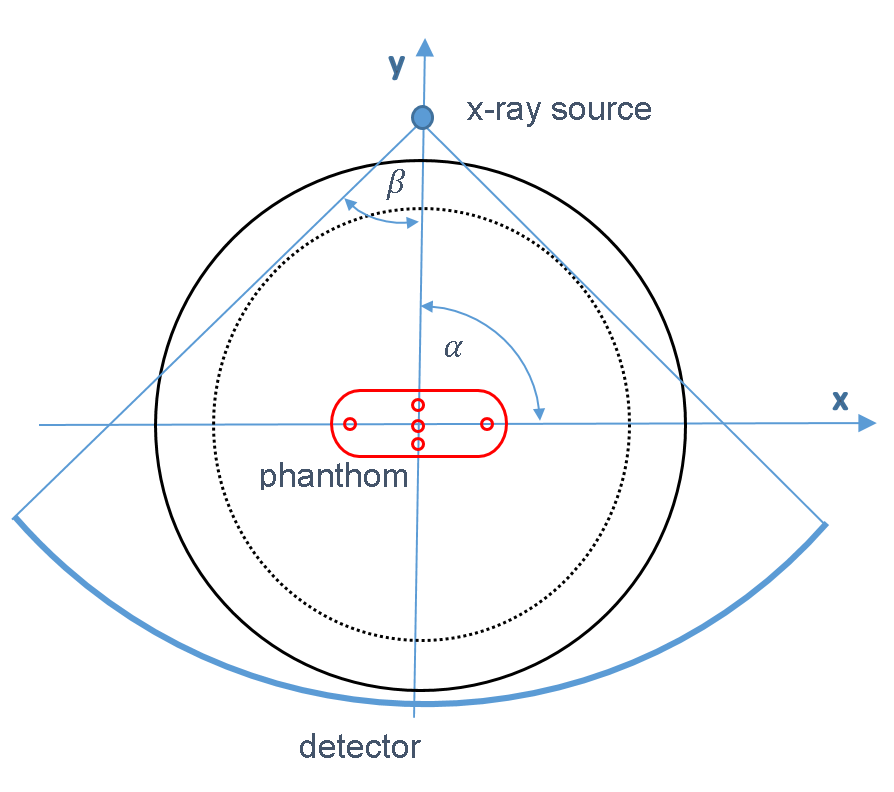
\includegraphics[scale=0.5]{pic01.png} \\

The diameter of scanned area is 500 mm. (Radius is 250 mm ) Distance from the isocenter to the x-ray source is 595 mm. We can calculate the angle $\beta$.\\
$\sin(\beta)=\frac{250}{595}$\\
$\beta=\arcsin{\frac{250}{595}}=$\\
$\beta=\arcsin{\frac{250}{595}}=\arcsin{0.420168}=24.85^{\circ}$\\
The scanning area is from $-\beta=-24.85^{\circ}$ to $+\beta=+24.85^{\circ}$  \\

Now we can express dimensions of the phantom as a function of $z$.\\
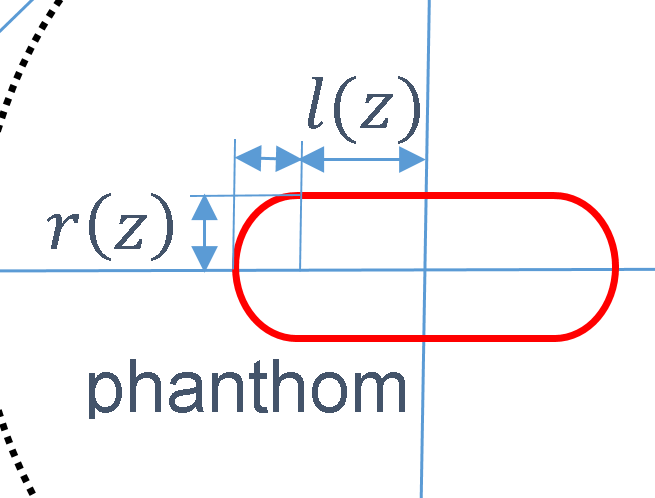
\includegraphics[scale=0.5]{pic01a.png}\\
Because $r(0)=40$ and $r(300)=80$ then $r(z)=40+\frac{80-40}{300}z=40+\frac{40}{300}z=40+\frac{4}{30}z$.\\
And from $l(0)=20$ and $l(300)=100$ follows $l(z)=20+\frac{100-20}{300}z=20+\frac{80}{300}z=20+\frac{8}{30}z$.\\

The width of the phantom is $2l(z)+2r(z)$ for any $z$ form 0 to 300.\\ 
The height of the phantom is $2r(z)$ for any $z$ form 0 to 300. \\
\section{Field of view}

The $(x,y)$ position of the x-ray source is determined by angle $\alpha$.\\
$Sx(\alpha)=595\sin{\alpha}$\\
$Sy(\alpha)=595\cos{\alpha}$\\
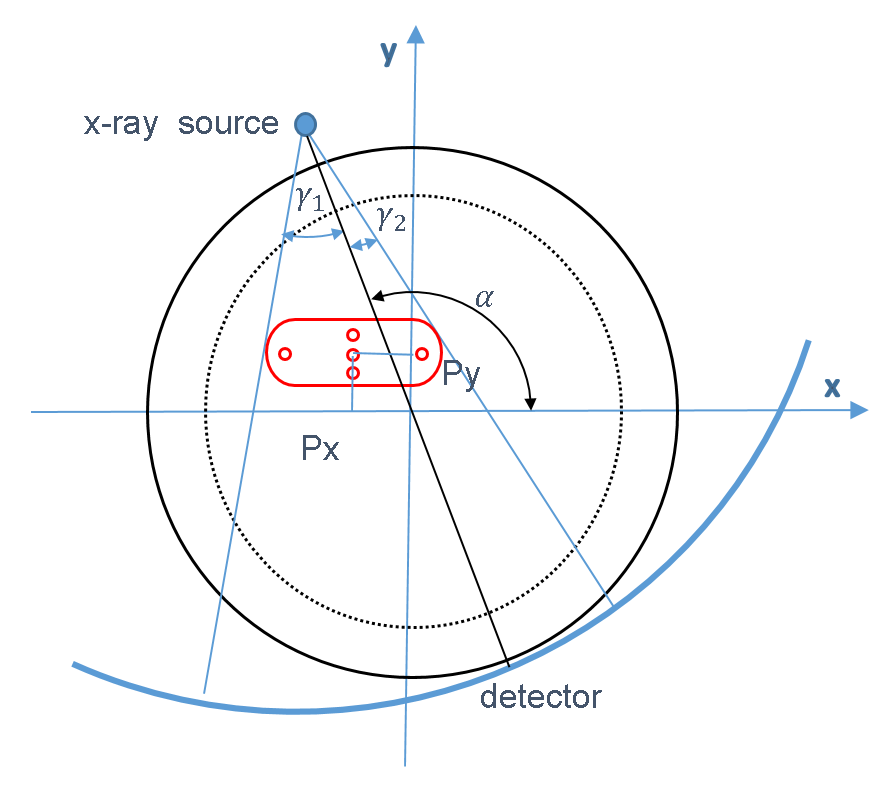
\includegraphics[scale=0.5]{pic02.png}\\
Constants are $Px=0, Py=0, Rs=595 mm$ \\
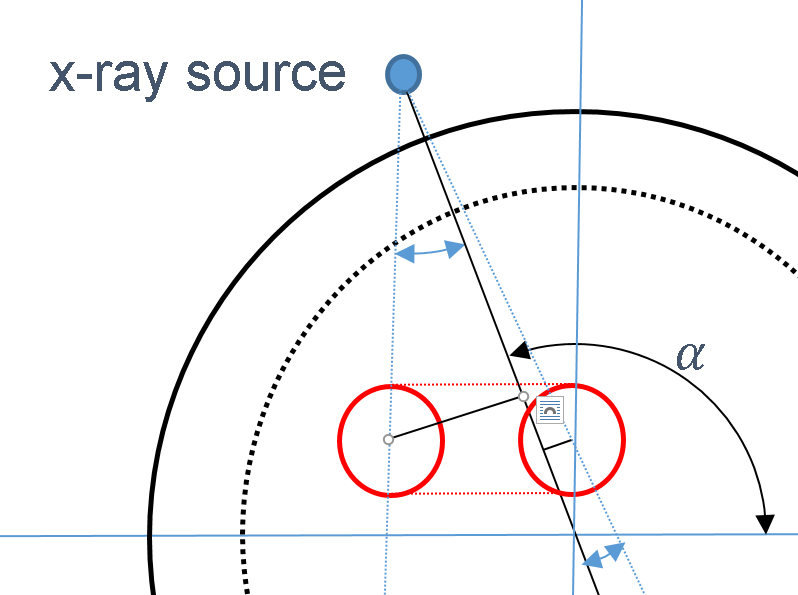
\includegraphics[scale=0.5]{pic03.png}\\
What are the $(x,y)$ coordinates of the center of the two circles.\\
One is $(Px-l(z),Py)$ and another one center is at $(Px+l(z),Py)$.\\

The straight line going thought "x-ray source" $(Sx,Sy)$ and isocenter $(0,0)$.\\
Direction vector is $(0,0)-(Sx,Sy)=(-Sx,-Sy)=(-595\sin{\alpha},-595\cos{\alpha})$.\\
The unit direction vector is  $(-\sin{\alpha},-\cos{\alpha})$. \\
Rotating this vector by $90^{\circ}$ counter clockwise (rotation formula (x,y) to (-y,x)) we will get the normal vector.\\
the unit normal vector $(\cos{\alpha},-\sin{\alpha})$\\

By doing scalar product of the normal vector with vectors from "x-ray source" to the center of the circle we will get distance of the center to the line.
By dividing those distances with distances from "x-ray source" to the center of the circles we will get $\sin$ of the angles.
Calculating $\arcsin$ of the $\sin$ of the angles we will get angles.\\

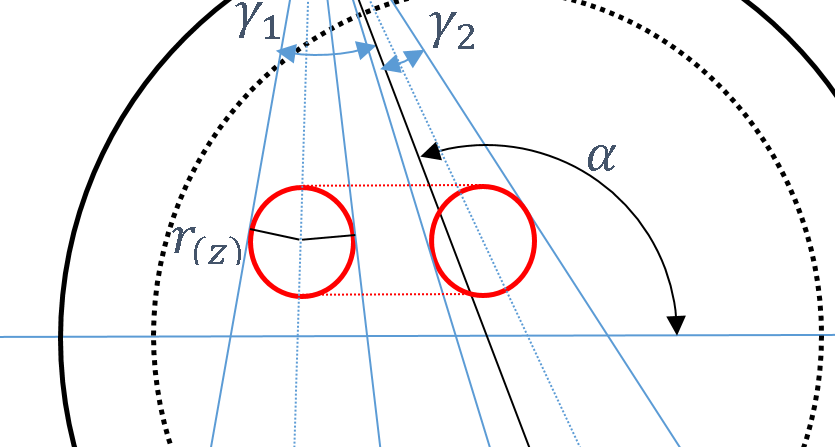
\includegraphics[scale=0.5]{pic04.png}\\

By using two angles from the previous step we will get 4 angles.

Minimum of those 4 we will named as $\gamma_1$ and maximum as  $\gamma_2$.\\
If $\gamma_1$ is less than $-\beta$ then $\gamma_1=-\beta$.\\
If $\gamma_2$ is greater than $\beta$ then $\gamma_2=\beta$.\\


\section{The length of the intersection}
This part is about finding three things . The last is "The length of the intersection"
\subsection{Find the intersection with the scanned area}
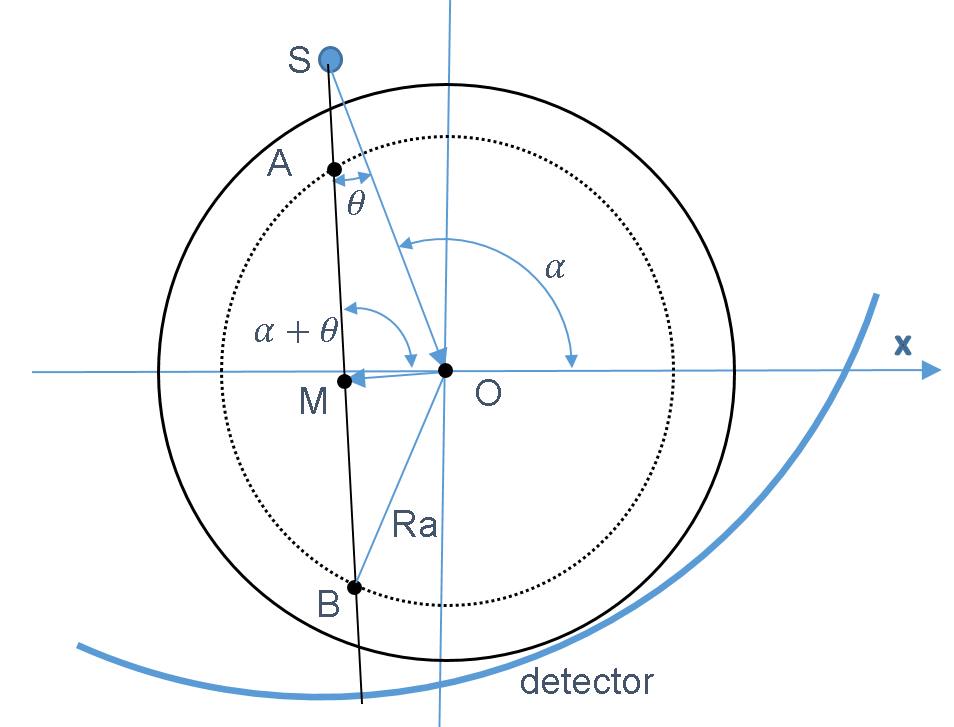
\includegraphics[scale=0.5]{pic05.png}\\
The unit normal vector of the straight line going though the points $S,A,M,B$ is \\
$\overrightarrow{n}=(\sin(-\alpha-\theta+90^{\circ}),\cos(-\alpha-\theta+90^{\circ}))$ \\
$\lvert OM \rvert=\Braket{\overrightarrow{n},\overrightarrow{SO}}$\\

If $\lvert OM \rvert$ is bigger than $Ra=250 mm$ "error"\\
$M=\lvert OM \rvert \cdot \overrightarrow{n}$\\
$\lvert MB \rvert =\sqrt{{Ra}^2-\lvert OM \rvert^2}$\\

$\overrightarrow{d}=(\sin(-\alpha-\theta),\cos(-\alpha-\theta))$ \\
$ B=M+\lvert MB \rvert \cdot \overrightarrow{d}$\\
$ A=M-\lvert MB \rvert \cdot \overrightarrow{d}$\\

\subsection{Find the point inside the phantom}
If point A is inside the phantom then C=A.
If point B is inside the phantom then D=B.
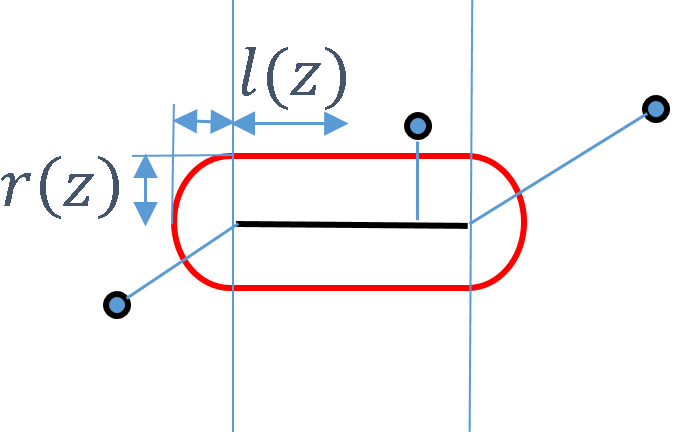
\includegraphics[scale=0.5]{pic06.png}\\
The point is inside the phantom if the distance from the straight line segment \\
from $(Px-l(z),Py)$  to  $(Px+l(z),Py)$ \\
is less or equal $r(z)$ \\
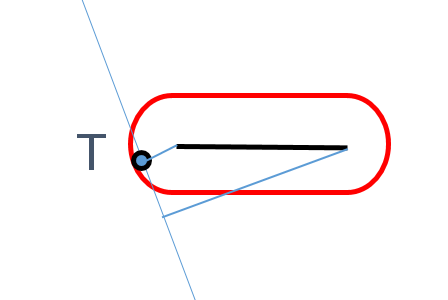
\includegraphics[scale=0.5]{pic07a.png}\\
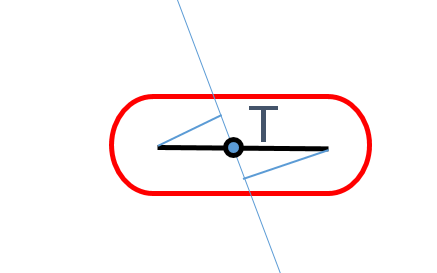
\includegraphics[scale=0.5]{pic07b.png}\\
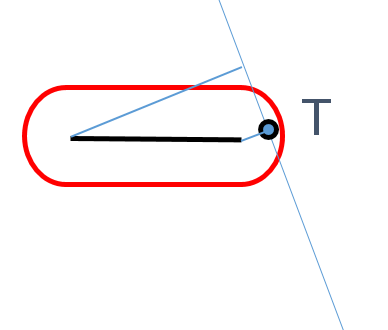
\includegraphics[scale=0.5]{pic07c.png}\\


\subsection{Find the points on the edge of the phantom}
By using Bisection method ...\\
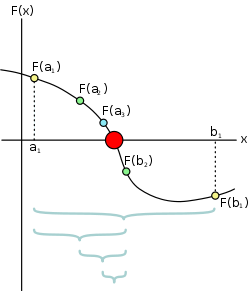
\includegraphics[scale=0.5]{Bisection_method.png}\\
-for points T and A we will get point C.\\
-for points T and B we will get point D.\\

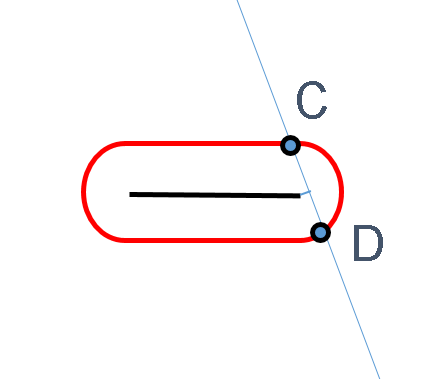
\includegraphics[scale=0.5]{pic08.png}\\
\section{Scanning the phantom}

The phantom is divided on 60 slices\\
1. from 0 to 5 mm ... this slice should be scanned at z=2.5 mm\\
2. from 5 to 10 mm ... this slice should be scanned at z=7.5 mm\\
3. from 10 to 15 mm ... this slice should be scanned at z=12.5 mm\\
...\\
60. from 295 to 300 mm ... this slice should be scanned at z=297.5 mm\\

\end{document}